\chapter{Tools}
\label{chapter:tools}


\section{Web Development Languages}

\begin{table}[ht]
\centering
\caption{Ranking among the most used languages on GitHub \parencite{stateOfTheOctoverse23}}
\label{tab:githubMostUsedLanguageRanking23}
\begin{tabular}[t]{|l|r|}
\toprule
Language & Rank\\
\midrule
JavaScript & 1\\
Python & 2\\
TypeScript & 3\\
C++ & 6\\
\bottomrule
\end{tabular}
\end{table}


\subsection{JavaScript}

A scripting language created by Brendan Eich in 1995 as part of the release of the \emph{Netscape 2} browser \parencite{javascriptRelease}, then was officially standardised by the Swiss standards body \emph{Ecma} in 1997 as \emph{ECMA-262} or \emph{ECMAScript}, as it is known today. This standard later was the basis for \emph{JScript} by \emph{Microsoft} and \emph{ActionScript} as part of \emph{Macromedia Flash}. The version currently being supported by all browsers (except Internet Explorer 11) is \ac{ES6} \parencite{javascriptHistory}.

\ac{JS} is an object-oriented, weakly-typed programming language that allows multiple programming paradigms to be applied. It is primarily used in the browser to add extra functionality to web pages. The underlying \emph{ECMAScript} standard does not define any input or output methods, which means that this is provided by the specific environment it is being used in (e.g. desktop or mobile browsers).

\subsection{TypeScript}

\ac{TS} was released by Microsoft in 2012 \textquote[\cite{typescriptRelease}]{to accommodate an increasing number of developers who are interested in using JavaScript to build large-scale Web applications to run in a browser rather than on the desktop.} It complies with the underlying Ecma scripting standard and is designed as a superset of \ac{JS}, adding static typing. It uses a compiler to generate regular \ac{JS} code.


\section{Native Application Development}

\subsection{Node JS}

Released initially by developer Ryan Dahl in 2009, a server-side \ac{JS} environment, Node.js runs standard ECMAScript in Google's V8 engine, allowing multithreading and native code integration. Its development was sponsored by the company Joyent. After some dissatisfaction in the community about Joyent's stewardship and a fork of Node.js called io.js. These difference were eventually resolved and everything was merged under the umbrella of the OpenJS Foundation. 

Node.js uses the \ac{NPM} to package code as modules, which can be used as dependencies. These modules can also integrate native C++ code, enabling bindings to most open-source libraries in the Linux ecosystem. It can be used to develop \ac{API}s or other server-side applications and support local web development processes like preprocessing, packaging, and deployment. 

\subsection{Python}

Guido van Rossum created the Python programming language in 1990 \parencite{pythonHistory}. It is a multi-paradigm language that is both dynamically and strongly typed \parencite{pythonTyping}. It relies heavily on indentation and whitespace to structure the code.

The language uses a standard library, and the surrounding ecosystem of available modules and applications based on Python makes it a good choice for data processing and science.

There is a native code interface that allows extending Python with bindings to native code, like with Node.js.

\subsection{C/C++}

C++ originated as an extension to C in 1985. It is a multi-paradigm, statically typed and object-oriented programming language.

It can be used to develop code for embedded platforms like Arduino, extend both Node.js and Python and, more generally, provide direct interaction with the operating system and its APIs.


\section{Frontend Frameworks and Libraries}

There is a wide range of available \ac{JS} frameworks to build dynamic frontends for \ac{SPA}s and \ac{PWA}s. The three libraries currently dominating the landscape are \emph{React}, developed by \emph{Facebook} in 2013, and \emph{Vue.js}, created by Evan You in 2014. These libraries can be used with frameworks to offer complete routing and state management solutions. Another popular framework is \emph{Angular}, initially released by \emph{Google} in 2010 and re-released in 2016.

\begin{figure}[h]
    \centering
    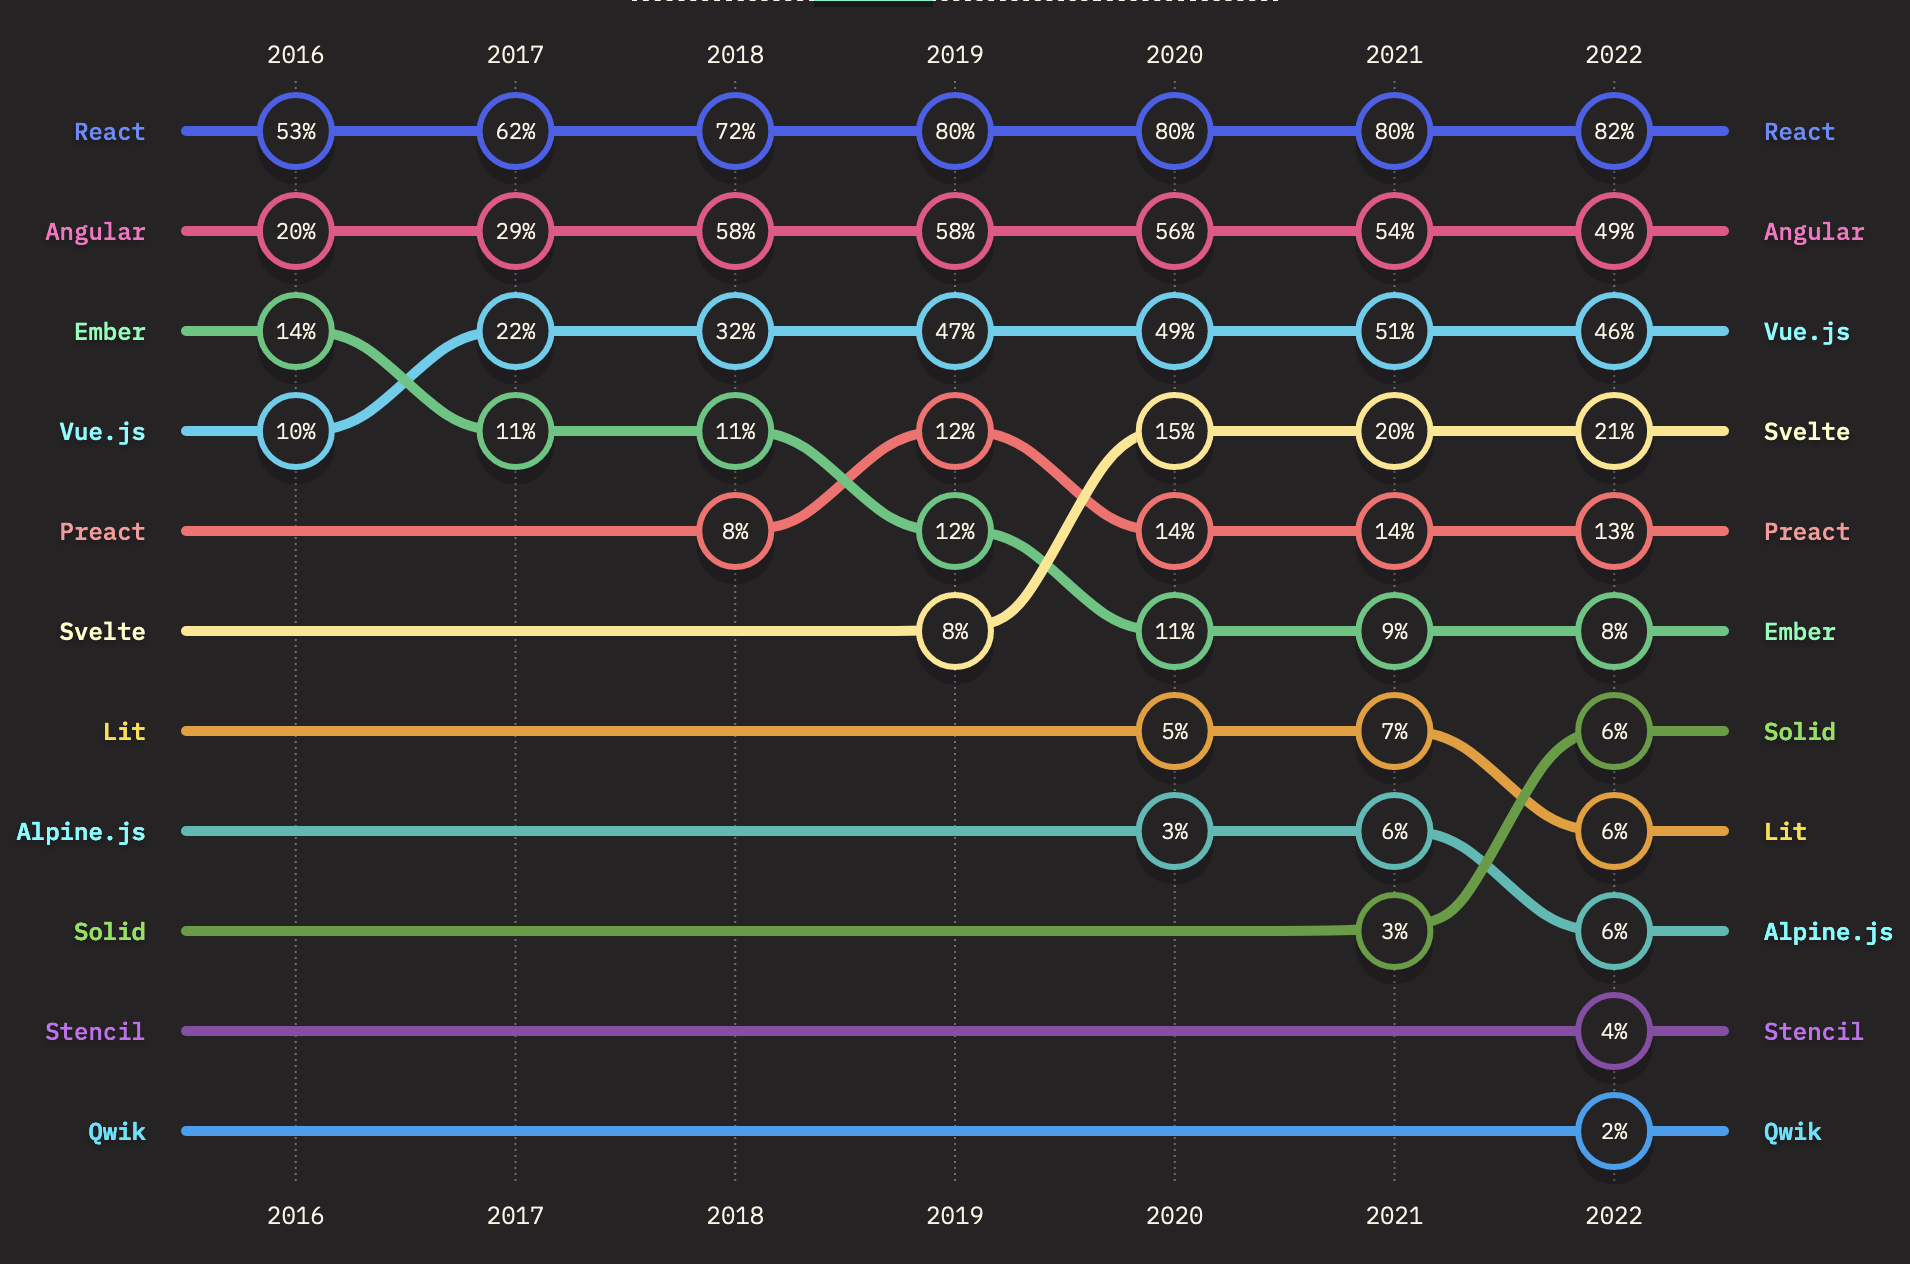
\includegraphics[scale=0.4]{04_Artefakte/01_Abbildungen/stateofjs-usage-frontend-frameworks-2022}
    \caption[{Most used frontend frameworks in 2022}]{State of JS: Most used frontend frameworks in 2022\protect\footnotemark}
    \label{fig:mostUsedFrameworks}
\end{figure}
\footnotetext{\cite{mostUsedFrontendFrameworks22}}

\subsection{React}

\emph{React} (\url{https://react.dev/}), developed by \emph{Facebook} and maintained by its successor \emph{Meta}, has become the most widely used tool for building \ac{SPA}s and is steadily leading the rankings for most used frontend frameworks both in the \emph{StackOverflow} \parencite{stackOverflowPollWebFrameworks23} and the \emph{State Of JS} \parencite{mostUsedFrontendFrameworks22} polls. By definition, it is not a framework but a \ac{UI} library that builds on other extensions to support state management, routing and deployment functionality. Although it is not a framework itself, there are existing frameworks like \emph{Next.js} (\url{https://nextjs.org/}) for the web and \emph{ReactNative} (\url{https://reactnative.dev/}) for building mobile apps using native functionality. React makes use of \ac{JSX}, which allows directly mixing inline \ac{HTML} with the \ac{JS} or \ac{TS} code structure.

\subsection{Vue.js}

\emph{Vue.js} (\url{https://vuejs.org/}) was developed by Evan You and is maintained by an international team of individuals. It had a relatively marginal presence in the US and Europe in the first years after its inception. This can be partially attributed to its origin in China, as most of its supporting modules were localised in Chinese. Over the years, it grew in popularity and received much more international support, eventually overcoming the language barrier. Unlike \emph{React}, it is billed as a "progressive framework" that provides fundamental functionality for building reactive components but also accommodates more complex use-cases \parencite{vueProgressiveFramework}. \emph{Vue.js} builds on standard \ac{JS} or \ac{TS}, \ac{HTML} and \ac{CSS} to build components, recommending a simple template mechanism mixed with reactive substitutions. However, it also supports using \ac{JSX} for specifying inline \ac{HTML} within \ac{JS}. As with \emph{React}, there are extensions and frameworks like \emph{Quasar} (\url{https://quasar.dev/}) and \emph{Nuxt} (\url{https://nuxt.com/}) that enable even more sophisticated workflows for application development and deployment.

\subsection{Angular}

\emph{Angular} was initially released by \emph{Google} in 2010 as \emph{AngularJS}  and officially discontinued in 2022 (\url{https://angularjs.org/}). A completely overhauled and currently used version 2 was released in 2016 and maintained by \emph{Google}. It is different from \emph{React} and \emph{Vue.js} in that it is a complete framework that contains everything required to build and deploy an application, and it explicitly recommends \ac{TS} as a programming language. The framework is also less flexible in that it is opinionated and has its own set of best practices baked into the framework's structure.




\section{Backend Libraries}

\subsection{Express}

The Express JS framework provides the basic functionality to create web servers including routing and middleware functionality. It was developed by TJ Holowaychuk, then sold to StrongLoop, which was subsequently acquired by IBM. It is currently under the stewardship of the OpenJS Foundation.

Express has become the de facto standard for building web services in JS, leading the ranking in the State of JS survey \parencite{mostUsedBackendFrameworks22}. Although it contains the necessary parts to build a web service, it does not enforce a specific architecture, which can be a problem for maintaining a robust application structure. For developers who prefer a more explicit structure, there are various other frameworks building on top of it and adding more opinionated structure or extensions.

\subsection{Koa}

Billed as a successor to Express, Koa is developed by the team behind Express. It aims to provide a more robust and minimalistic iteration on the middleware-based architecture of Express. Like Express, it allows for building a service from scratch in completely free form, but is also the basis for other, more explicitly structured frameworks.


\section{Backend Frameworks}

For more complex applications a more stringent and structured application structure, other frameworks might be more desirable. There are numerous \ac{JS} frameworks, some based on Express or Koa, others provide their own basis for routing. To review all possible options is beyond the scope of this study. In the following, three frameworks are selected for their specific nature related to popularity, stability but also with an explicit focus on real-time applications.

\begin{table}[ht]
\centering
\caption{State of JS survey: Most used backend frameworks \parencite{mostUsedBackendFrameworks22}}
\label{tab:backendFrameworksRanking}
\begin{tabular}[t]{lcc}
\toprule
Framework & \% of question respondents\\
\midrule
Nest & 30.2\\
Feathers & 8.8\\
Meteor & 2.7\\
\bottomrule
\end{tabular}
\end{table}


\subsection{Nest JS}

Nest JS is a backend framework for developers who look for a more strictly opinionated and robust setup than Express, e.g. for enterprise applications. It follows a modular concept, making dependencies available to the services via injection, there are multiple database options and transports can be both HTTP and WebSockets. There are \ac{CLI} scripts that enable automatic generation of boilerplate application code and the language used to build Nest applications is TypeScript. It scores the second rank among the most-used backend frameworks in the State of JS survey \parencite{mostUsedBackendFrameworks22}.

\subsection{Feathers}

This framework takes a very different approach in that it makes very little assumptions about the specific application structure. It uses aspect-oriented programming and uses a service-centric architecture. The usage of before-, after- and around-hooks (so called \textquote{cross-cutting concerns}) for the services that modify basic behaviour or add functionality. There are adapters for a wide range of databases and authentication methods. The framework has a dedicated concept of channels that enable real-time functionality and messaging to clients. Real-time transports are also abstracted and can be deployed using various different WebSockets libraries. It also provides a \ac{CLI} to generate application code that can be written in \ac{JS} or \ac{TS}.

Feathers started as a hobby project by David Luecke and Eric Kryski in 2013 \parencite{feathersFrameworkHistory} and is currently maintained by David Luecke and a community of individual contributors. In the State of JS survey, it is still in the lower percentages, but almost doubled that percentage from the previous survey in 2021 \parencite{mostUsedBackendFrameworks21}.

\subsection{Meteor}

Meteor focuses explicitly on real-time applications using WebSockets. The framework is a bit of an outlier in that its core is open-source, but other parts are proprietary code. Nonetheless, it should be mentioned, because it has been around for over ten years and it uses WebSockets exclusively. It was released in 2012 by a startup company, immediately received venture capital funding by Andreesen Horowitz and was eventually sold again in 2019.

The framework primarily uses MongoDB as a database system, provides its own package manager and ecosystem, its own build system and template system based on Mustache.
